\documentclass[12pt, border=8pt]{standalone}
\usepackage{tikz}
\usepackage{amsmath, amssymb, bm}
\usepackage{xcolor}
\usepackage{booktabs}
\usetikzlibrary{positioning, arrows.meta, calc, fit, backgrounds, 3d}

\begin{document}


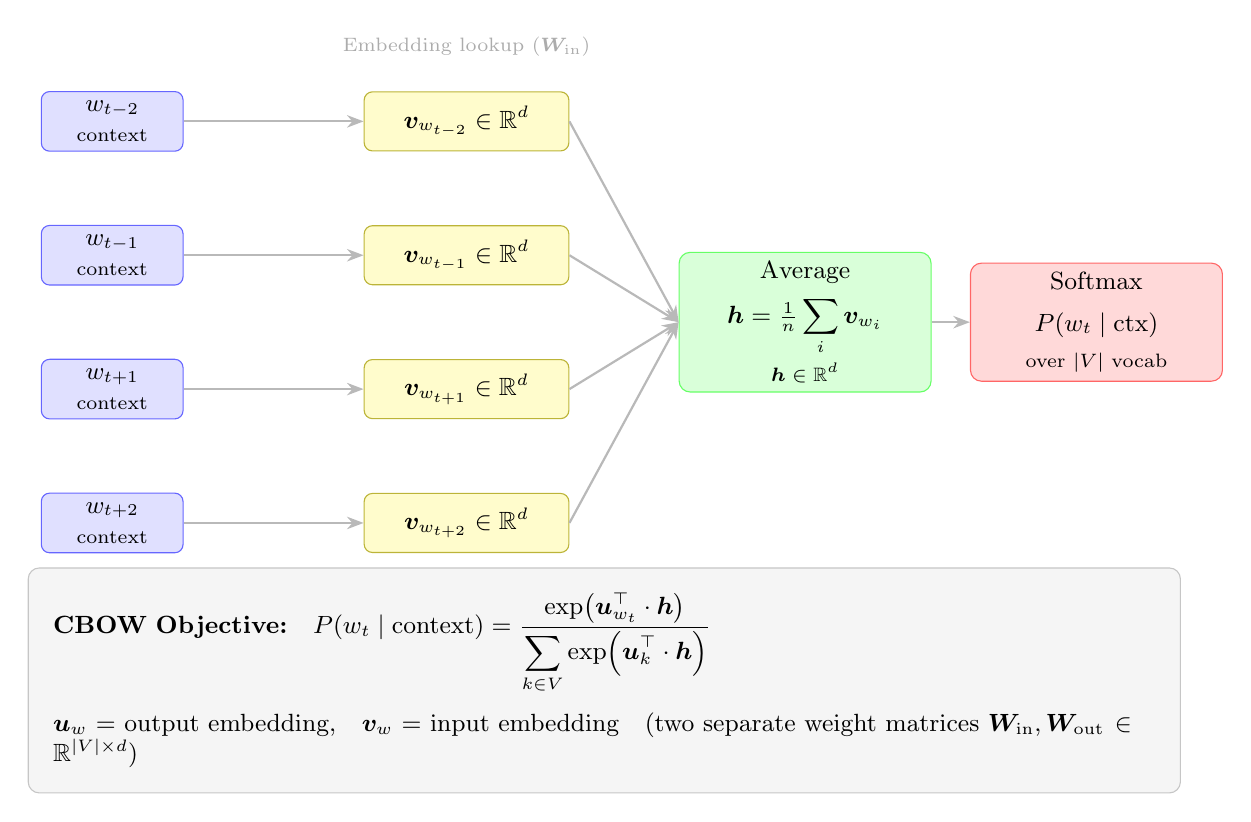
\begin{tikzpicture}[
  every node/.style={font=\small},
  arr/.style={-{Stealth[length=6pt]}, thick, gray!55},
  ctxbox/.style={draw=blue!60, fill=blue!12, rounded corners=3pt,
                 minimum width=1.8cm, minimum height=0.75cm, align=center, font=\small},
  embbox/.style={draw=yellow!70!black, fill=yellow!20, rounded corners=3pt,
                 minimum width=2.6cm, minimum height=0.75cm, align=center, font=\small},
  avgbox/.style={draw=green!60, fill=green!15, rounded corners=4pt,
                 minimum width=3.2cm, minimum height=1.5cm, align=center, font=\small},
  smbox/.style={draw=red!60, fill=red!15, rounded corners=4pt,
                minimum width=3.2cm, minimum height=1.3cm, align=center, font=\small}
]

% ---- Context word boxes (left column) ----
\node[ctxbox] (w1) at (0, 3.3)   {$w_{t-2}$\\{\scriptsize context}};
\node[ctxbox] (w2) at (0, 1.6)   {$w_{t-1}$\\{\scriptsize context}};
\node[ctxbox] (w3) at (0,-0.1)   {$w_{t+1}$\\{\scriptsize context}};
\node[ctxbox] (w4) at (0,-1.8)   {$w_{t+2}$\\{\scriptsize context}};

% ---- Embedding lookup boxes (middle column) ----
\node[embbox] (e1) at (4.5, 3.3)   {$\bm{v}_{w_{t-2}} \in \mathbb{R}^d$};
\node[embbox] (e2) at (4.5, 1.6)   {$\bm{v}_{w_{t-1}} \in \mathbb{R}^d$};
\node[embbox] (e3) at (4.5,-0.1)   {$\bm{v}_{w_{t+1}} \in \mathbb{R}^d$};
\node[embbox] (e4) at (4.5,-1.8)   {$\bm{v}_{w_{t+2}} \in \mathbb{R}^d$};

% Label above embedding column
\node[font=\scriptsize, text=gray!65] at (4.5, 4.25) {Embedding lookup ($\bm{W}_{\text{in}}$)};

% ---- Average box ----
\node[avgbox] (avg) at (8.8, 0.75)
  {Average\\[4pt]
   $\bm{h} = \tfrac{1}{n}\displaystyle\sum_i \bm{v}_{w_i}$\\[2pt]
   {\scriptsize $\bm{h} \in \mathbb{R}^d$}};

% ---- Softmax box ----
\node[smbox] (sm) at (12.5, 0.75)
  {Softmax\\[4pt]
   $P(w_t \mid \text{ctx})$\\[2pt]
   {\scriptsize over $|V|$ vocab}};

% ---- Arrows: context -> embedding ----
\foreach \i/\j in {w1/e1, w2/e2, w3/e3, w4/e4}
  \draw[arr] (\i.east) -- (\j.west);

% ---- Arrows: embedding -> avg ----
\foreach \j in {e1,e2,e3,e4}
  \draw[arr] (\j.east) -- (avg.west);

% ---- Arrow: avg -> softmax ----
\draw[arr] (avg.east) -- (sm.west);

% ---- Formula box ----
\node[draw=gray!45, fill=gray!8, rounded corners=4pt, align=left, font=\small,
      inner sep=9pt, text width=14cm] at (6.25,-3.8) {%
  \textbf{CBOW Objective:}\quad
  $P(w_t \mid \text{context}) =
   \dfrac{\exp\!\left(\bm{u}_{w_t}^\top \cdot \bm{h}\right)}
         {\displaystyle\sum_{k \in V} \exp\!\left(\bm{u}_k^\top \cdot \bm{h}\right)}$\\[6pt]
  $\bm{u}_w$ = output embedding,\quad
  $\bm{v}_w$ = input embedding\quad
  (two separate weight matrices $\bm{W}_{\text{in}}, \bm{W}_{\text{out}} \in \mathbb{R}^{|V|\times d}$)
};

\end{tikzpicture}

\end{document}
